\documentclass[11pt]{article}

\usepackage[margin=1in]{geometry}
\usepackage{amsmath,amssymb,amsthm}
\usepackage{booktabs}
\usepackage{enumitem}
\usepackage{graphicx}
\usepackage{hyperref}
\usepackage{natbib}

\newtheorem{theorem}{Theorem}
\newtheorem{lemma}{Lemma}
\newtheorem{assumption}{Assumption}
\newtheorem{definition}{Definition}
\newtheorem{proposition}{Proposition}
\newtheorem{remark}{Remark}

\title{Drift-Aware Spectral Conformal Prediction for Non-Exchangeable Streaming Data}
\author{
Jeffery Opoku\textsuperscript{1,*}
\and
David Banahene\textsuperscript{2}
\\[0.5em]
\textsuperscript{1}The University of Texas Rio Grande Valley, Edinburg, TX, USA\\
\textsuperscript{2}Florida International University, Miami, FL, USA\\
\textsuperscript{*}Corresponding author: \texttt{jeffery.opoku01@utrgv.edu}\\
David Banahene: \texttt{abanahene54@gmail.com}
}
\date{}

\begin{document}

\maketitle

\begin{abstract}
Conformal prediction provides distribution-free prediction intervals under exchangeability, but many modern data streams are neither independent nor stable. They exhibit recurring regimes, changing seasonal frequencies, abrupt shifts, and gradual drift. We propose drift-aware spectral conformal prediction (DASC), a streaming uncertainty quantification framework for structured non-exchangeable data subject to distributional drift. DASC forms conformal prediction intervals using calibration residuals weighted by local spectral similarity, while a transport-based drift score monitors whether the current test distribution has moved away from past calibration regimes. When drift is mild, DASC borrows calibration residuals from structurally similar historical windows; when drift is severe, it contracts or reweights the calibration pool and updates the target miscoverage level online. The method also reports an effective sample size diagnostic that warns when a weighted conformal quantile is statistically fragile. We establish an approximate coverage bound that decomposes coverage loss into drift, residual mismatch, and weighted effective sample size. In synthetic experiments and five stress-test regimes, DASC maintains near-nominal coverage after drift where rolling, recency-weighted, and spectral-only conformal methods can under-cover. In real electricity and weather streams, DASC reduces average interval width by approximately 28\% and 42\%, respectively, relative to the best calibrated non-DASC baseline, while preserving calibrated or conservative coverage. A financial volatility example shows a more nuanced regime in which spectral-only calibration is competitive, but DASC retains near-nominal coverage and adds drift diagnostics.
\end{abstract}

\noindent\textbf{Keywords and phrases:} conformal prediction; streaming data; distribution shift; optimal transport; spectral methods; adaptive conformal inference.

\medskip
\noindent\textbf{2020 Mathematics Subject Classification:} Primary 62G15; secondary 62M10, 62L12, 62G20.

\section{Introduction}

Conformal prediction has become one of the most attractive tools for uncertainty quantification because it can wrap around almost any prediction algorithm and produce prediction sets with finite-sample coverage under exchangeability \citep{vovk2005algorithmic,angelopoulos2021gentle}. This model-agnostic character is especially valuable in modern forecasting problems, where the point predictor may be a random forest, gradient boosting machine, recurrent neural network, transformer, or foundation model. The basic conformal promise is simple: after a calibration step, prediction intervals can be constructed with a user-specified coverage level without requiring a correctly specified parametric model.

The difficulty is that the cleanest conformal guarantees rely on exchangeability. In streaming applications, the observations are rarely exchangeable. Electricity demand, disease surveillance, climate measurements, traffic flows, financial volatility, and public health indicators all exhibit temporal dependence, seasonality, regime recurrence, local bursts, abrupt shifts, and gradual drift. The prediction error at time $t$ is often more closely related to selected historical periods than to the calibration sample as a whole. A calibration residual from last week's matching daily cycle may be informative, while a residual from an unrelated regime may be misleading. This creates a central problem for conformal prediction in time-indexed data: the method must decide which past residuals remain relevant to the current prediction.

Recent work has made substantial progress on conformal prediction for time series. Methods such as EnbPI construct sequential intervals without requiring full exchangeability and provide finite-sample or asymptotic coverage bounds under weaker time-series assumptions \citep{xu2020time}. Other approaches modify the conformal score, the calibration unit, or the prediction-set geometry to account for multistep dependence, multivariate outputs, functional time series, and temporal correlations \citep{sun2022copula,lee2025flow,cleaveland2023linear,xu2024ellipsoidal}. A related line of work uses modern sequence models, graph structure, or reservoir-style state representations to exploit temporal dependence when forming intervals \citep{auer2023hopfield,lee2024transformer,negli2025reservoir,cini2025relational}. These contributions show that time dependence is not merely a nuisance; it can be used as information for sharper uncertainty quantification.

A second line of work addresses adaptivity. Adaptive conformal inference updates the nominal miscoverage level online in response to realized coverage errors, giving methods that can maintain long-run calibration even when the data-generating process changes \citep{gibbs2021adaptive,zaffran2022adaptive}. Control-theoretic variants, including conformal PID control, provide another way to stabilize empirical coverage in sequential forecasting tasks affected by seasonality, trends, and distribution shifts \citep{angelopoulos2023pid}. Parameter-free and betting-based versions further reduce sensitivity to learning-rate choices in online adaptive calibration \citep{bastani2024betting}. These methods are powerful because they do not require a full model for the evolving data stream. However, adaptivity alone does not specify how to select the most relevant calibration residuals at a given time.

A third line of work studies conformal prediction under distribution shift. Weighted conformal prediction and covariate-shift methods modify the conformal quantile using importance weights or local relevance scores \citep{tibshirani2019conformal}. More recent work introduces robust conformal procedures for broader forms of distributional change, including Wasserstein-regularized conformal prediction, optimal-transport formulations for non-exchangeable data, and robustness under Levy-Prokhorov perturbations \citep{xu2025wasserstein,correia2025optimal,aolaritei2025levy}. These papers are especially relevant for streaming data because they provide language for comparing calibration and test distributions rather than assuming that the calibration sample remains representative.

Despite these advances, an important gap remains. Time-series conformal methods often exploit temporal structure but may not explicitly measure when that structure has drifted away from the calibration history. Adaptive conformal methods can correct long-run coverage but may react only after errors have occurred. Distribution-shift methods can compare calibration and target distributions, but they are not always designed to exploit recurring spectral or seasonal structure in a data stream. In many applications, all three issues occur together: the data are non-exchangeable, the non-exchangeability has recurring structure, and the structure itself may drift.

This paper proposes drift-aware spectral conformal prediction (DASC) for this combined setting. The method begins from the idea that local frequency content provides a useful representation of structured non-exchangeability. A current test window is compared with historical calibration windows through spectral features such as smoothed periodograms, wavelet energies, or low-dimensional frequency summaries. Calibration residuals from spectrally similar windows receive larger weights. This spectral weighting allows the method to borrow information from recurring regimes even when those regimes are separated in calendar time.

Spectral similarity alone is not enough when the current stream enters a genuinely new state. Therefore, the second ingredient is a transport-based drift diagnostic. We compare the empirical distribution of the current window with the weighted empirical calibration distribution using a Wasserstein or entropic optimal-transport discrepancy. The resulting drift score measures whether the spectrally selected calibration residuals plausibly represent the current regime. When the drift score is small, the method trusts spectrally similar historical residuals; when the score is large, it contracts or tempers the calibration pool and relies more heavily on recent data.

The third ingredient is adaptive conformal calibration. After each response is observed, the method updates the target miscoverage level according to the realized coverage error. This online update provides a correction mechanism when the weighted quantile is temporarily miscalibrated. The resulting procedure combines prospective similarity search, distributional drift monitoring, and retrospective coverage correction.

The practical question addressed by this paper is therefore the following: when should a streaming conformal predictor trust structurally similar past data, and when should it treat the present as a new regime? The proposed answer is to use spectral features to identify recurring structure, transport discrepancy to monitor whether that structure remains distributionally reliable, and adaptive calibration to maintain long-run coverage.

\paragraph{Contributions.}
This paper makes four contributions.
\begin{enumerate}[label=(\roman*)]
    \item We introduce DASC, a drift-aware spectral weighting scheme for conformal prediction in non-exchangeable streaming data.
    \item We define a drift diagnostic based on discrepancy between the current window and the weighted calibration distribution.
    \item We combine the weighted conformal quantile with an adaptive miscoverage update that targets long-run calibration.
    \item We report an effective sample size diagnostic that indicates when a locally weighted conformal threshold is reliable enough to use.
    \item We evaluate the method on synthetic streams with recurring regimes, abrupt shifts, gradual drift, heavy tails, weak recurrence, and three real data examples.
\end{enumerate}

\paragraph{Main findings.}
The main findings are as follows.
\begin{enumerate}[label=(\roman*)]
    \item DASC separates reliability into three quantities that can be inspected in practice: coverage error, transport drift, and effective sample size.
    \item Spectral-only and recency-weighted conformal calibration can work in recurring regimes but fail sharply after distributional drift.
    \item The drift gate improves the theoretical coverage-loss bound when the reduction in drift bias is larger than the increase in weighted-quantile variability.
    \item In household electricity and hourly weather data, DASC reduces average interval width by approximately $28\%$ and $42\%$, respectively, relative to the best calibrated non-DASC baseline.
    \item In financial volatility, DASC remains near nominal coverage and provides diagnostics, while spectral-only weighting remains competitive in interval width.
\end{enumerate}

\section{Related Work}

The present paper is connected to four strands of literature: conformal prediction for time series, adaptive online conformal calibration, conformal prediction under distribution shift, and representation-based calibration for dependent data.

\paragraph{Conformal prediction for time series.}
Classical conformal prediction gives finite-sample marginal coverage when the calibration and test observations are exchangeable \citep{vovk2005algorithmic,angelopoulos2021gentle}. Since time-series observations are temporally dependent, a growing literature has developed conformal methods that modify either the calibration scheme or the prediction-set geometry. \citet{xu2020time} proposed EnbPI, a sequential method that avoids full retraining and gives distribution-free prediction intervals for time series under weaker assumptions than exchangeability. Other work has extended conformal time-series methods to multi-step forecasting, functional observations, multivariate outputs, and non-rectangular prediction regions \citep{sun2022copula,cleaveland2023linear,xu2024ellipsoidal,lee2025flow}. These papers demonstrate that temporal dependence can be handled by redesigning the calibration unit, the nonconformity score, or the geometry of the prediction region.

Our work differs in emphasis. Instead of treating dependence only as an obstacle to validity, we use local spectral structure as a way to identify relevant calibration residuals. This is most useful in streams with recurring regimes, where calendar proximity is not the only marker of relevance. A residual from a distant but spectrally similar period may be more informative than a recent residual from a different regime.

\paragraph{Adaptive and online conformal calibration.}
Adaptive conformal inference updates the calibration threshold or nominal miscoverage level as new observations arrive. \citet{gibbs2021adaptive} introduced an online update that adjusts the target miscoverage level in response to realized coverage errors, and \citet{zaffran2022adaptive} studied adaptive conformal prediction in time-series settings. Control-inspired methods such as conformal PID control use proportional, integral, and derivative feedback to stabilize coverage in sequential forecasting problems affected by seasonality, trends, and distribution shifts \citep{angelopoulos2023pid}. More recent parameter-free approaches, such as betting-based adaptive conformal inference, reduce dependence on manually tuned learning rates while preserving long-run calibration behavior \citep{bastani2024betting}.

These adaptive methods are important because they make few assumptions on the data-generating process. Their limitation is that they are often reactive: the update responds after miscoverage has already occurred. In streaming applications with abrupt or gradual drift, it is useful to have a prospective diagnostic that asks whether the current regime still resembles the weighted calibration distribution. Our method keeps the adaptive update but supplements it with a transport drift score that can change the calibration weights before coverage errors accumulate.

\paragraph{Distribution shift, weighting, and transport.}
Weighted conformal prediction addresses settings in which the calibration distribution and test distribution differ in a structured way. Under covariate shift, for example, calibration residuals can be reweighted using likelihood or density-ratio information \citep{tibshirani2019conformal}. Recent work has expanded this idea to broader shift models. Wasserstein-regularized conformal prediction uses optimal-transport style constraints to obtain robustness under distributional perturbations \citep{xu2025wasserstein}. Non-exchangeable conformal prediction with optimal transport uses unlabeled data to tackle distribution shifts between calibration and test samples \citep{correia2025optimal}. Related robustness frameworks study coverage under Levy-Prokhorov perturbations, giving another way to quantify local and global distributional changes \citep{aolaritei2025levy}.

This literature provides the formal language for measuring how far the current data distribution has moved from calibration. Our contribution is to make this comparison local and streaming: the transport discrepancy is computed between a current window and a weighted calibration distribution selected by spectral similarity. The transport score is not used alone as a worst-case robustness device; it is used operationally to decide how much to trust spectrally similar historical residuals.

\paragraph{Representation-based calibration.}
Another recent direction uses learned or engineered representations to improve conformal calibration under dependence. Hopfield-network conformal prediction, transformer conformal prediction, reservoir conformal prediction, and relational conformal prediction all use hidden states, learned attention, reservoir states, or graph structure to represent the relevant temporal context before constructing prediction intervals \citep{auer2023hopfield,lee2024transformer,negli2025reservoir,cini2025relational}. These methods share an important insight with the present paper: calibration residuals should be compared in a representation space that reflects the structure of the forecasting problem.

The representation used here is deliberately simple and interpretable. Local spectral features summarize frequency content, seasonality, and regime recurrence. Such features are natural in many scientific and economic time series, and they produce diagnostics that can be inspected directly. This is a useful complement to deep sequence representations, especially when the goal is not only predictive efficiency but also transparent uncertainty quantification.

\paragraph{Positioning of this paper.}
The proposed DASC method combines ideas from these four strands. From time-series conformal prediction, it inherits the goal of valid uncertainty quantification under dependence. From adaptive conformal inference, it inherits online correction of long-run coverage. From distribution-shift conformal prediction, it borrows the use of weighted calibration and transport discrepancy. From representation-based calibration, it adopts the principle that relevance should be defined in a problem-specific feature space. The resulting procedure is designed for streams where non-exchangeability is structured, recurring, and drifting.

\paragraph{Scope of the present comparison.}
The experiments in this paper are intended to isolate the value of spectral weighting, drift gating, and adaptive calibration. For that reason, the main comparisons use transparent baselines: rolling conformal prediction, adaptive conformal inference, conformal PID, spectral-only conformal prediction, and ablated versions of DASC. More complex methods such as EnbPI, AgACI, transformer conformal prediction, and reservoir conformal prediction are important benchmarks for a larger forecasting study, but they also introduce additional modeling choices. The present paper focuses on the calibration layer and uses simple forecasters so that differences in coverage and width can be attributed mainly to the conformal mechanism.

\section{Problem Setup}

Let $\{(X_t,Y_t)\}_{t\geq 1}$ be a streaming sequence, where $X_t$ denotes covariates or recent history and $Y_t$ is the response. Let $\widehat f_t$ be a prediction rule trained before observing $Y_t$, and let
\[
    R_t = |Y_t-\widehat f_t(X_t)|
\]
denote the conformity residual. For a target miscoverage level $\alpha\in(0,1)$, the goal is to construct an interval
\[
    C_t(X_t) = [\widehat f_t(X_t)-q_t,\widehat f_t(X_t)+q_t]
\]
such that the realized error indicators
\[
    E_t = \mathbf{1}\{Y_t\notin C_t(X_t)\}
\]
are controlled in a meaningful finite-sample or long-run sense, despite non-exchangeability.

\begin{table}[t]
\centering
\caption{Main notation.}
\label{tab:notation}
\begin{tabular}{ll}
\toprule
Symbol & Meaning \\
\midrule
$X_t,Y_t$ & Covariates/history and response at time $t$ \\
$\widehat f_t$ & Point forecaster used before observing $Y_t$ \\
$R_t$ & Nonconformity residual, usually $|Y_t-\widehat f_t(X_t)|$ \\
$\alpha$ & Target miscoverage level \\
$\alpha_t$ & Adaptive miscoverage level at time $t$ \\
$C_t(X_t)$ & Prediction interval at time $t$ \\
$\mathcal{C}_t$ & Calibration pool available before time $t$ \\
$W_t$ & Local window around prediction time $t$ \\
$S_t=\Phi(W_t)$ & Spectral feature vector for window $W_t$ \\
$w_{i,t}$ & Final calibration weight assigned to residual $R_i$ \\
$\widehat F_{w,t}$ & Weighted empirical calibration residual distribution \\
$F_t$ & Conditional residual distribution at time $t$ \\
$D_t$ & Transport drift score between current and calibration distributions \\
$n_{\mathrm{eff},t}$ & Effective sample size, $1/\sum_i w_{i,t}^2$ \\
$m_t(D_t)$ & Drift-gated calibration window length \\
$\delta_t$ & Residual mismatch not explained by the drift score \\
$L_t$ & Local constant linking drift score to calibration bias \\
\bottomrule
\end{tabular}
\end{table}

\section{Spectral Features}

For each time $t$, let $W_t$ denote a local window ending near $t$. We compute a spectral feature vector
\[
    S_t = \Phi(W_t),
\]
where $\Phi$ may be a periodogram, smoothed power spectrum, wavelet energy vector, or low-dimensional frequency summary. The spectral distance between a calibration time $i$ and test time $t$ is
\[
    d_{\mathrm{spec}}(i,t) = \|S_i-S_t\|_2.
\]
The corresponding spectral weight is
\[
    w^{\mathrm{spec}}_{i,t}
    =
    \frac{\exp\{-d_{\mathrm{spec}}(i,t)^2/h_t^2\}}
    {\sum_{j\in \mathcal{C}_t}\exp\{-d_{\mathrm{spec}}(j,t)^2/h_t^2\}},
\]
where $\mathcal{C}_t$ is the calibration pool and $h_t>0$ is a bandwidth.

\section{Transport Drift Diagnostic}

Let $\widehat P_t$ denote the empirical distribution of recent observations or residual-feature pairs in a current window. Let $\widehat Q_t$ denote the weighted empirical calibration distribution induced by the spectral weights. We define a drift score
\[
    D_t = \mathcal{W}_p(\widehat P_t,\widehat Q_t),
\]
where $\mathcal{W}_p$ is a Wasserstein distance or an entropically regularized optimal transport discrepancy.

Large values of $D_t$ indicate that the current stream is poorly represented by the weighted calibration distribution. The drift score is used to temper the spectral weights or contract the calibration pool.

\section{Drift-Aware Spectral Conformal Prediction}

This section defines DASC as an operational algorithm. At each time $t$, the method computes spectral features for the current window, assigns calibration weights to past residuals, measures drift between the current window and the weighted calibration distribution, adjusts the calibration pool if drift is large, computes a weighted conformal quantile, and then updates the target miscoverage level after the response is observed.

\paragraph{Algorithm: DASC.}
For each prediction time $t$:
\begin{enumerate}[label=\arabic*.]
    \item Form a current window $W_t$ and compute its spectral feature vector $S_t=\Phi(W_t)$.
    \item For each calibration index $i\in\mathcal{C}_t$, compute $S_i=\Phi(W_i)$ and the spectral distance $d_{\mathrm{spec}}(i,t)$.
    \item Construct preliminary spectral weights $w^{\mathrm{spec}}_{i,t}$.
    \item Compute the transport drift score $D_t=\mathcal{W}_p(\widehat P_t,\widehat Q_t)$ between the current empirical distribution and the weighted calibration distribution.
    \item Use $D_t$ to choose a drift-gated calibration window or drift-tempered weights.
    \item Compute the effective sample size $n_{\mathrm{eff},t}=1/\sum_i w_{i,t}^2$.
    \item Compute the weighted conformal quantile $q_t$ at level $1-\alpha_t$ and return the interval $C_t(X_t)$.
    \item After observing $Y_t$, update $\alpha_t$ using the realized miss indicator $E_t=\mathbf{1}\{Y_t\notin C_t(X_t)\}$.
\end{enumerate}

\begin{center}
\fbox{
\begin{minipage}{0.94\textwidth}
\textbf{Algorithm 1: Drift-Aware Spectral Conformal Prediction (DASC)}

\vspace{0.5em}
\textbf{Input:} calibration pool $\mathcal{C}_t$, residuals $\{R_i:i\in\mathcal{C}_t\}$, spectral map $\Phi$, bandwidth $h_t$, drift threshold $\lambda_t$, target level $\alpha_t$, minimum and maximum window sizes $m_{\min},m_{\max}$.

\vspace{0.5em}
\textbf{For each prediction time $t$:}
\begin{enumerate}[label=\arabic*.]
    \item Compute the current spectral feature $S_t=\Phi(W_t)$ and historical features $S_i=\Phi(W_i)$ for $i\in\mathcal{C}_t$.
    \item Form preliminary spectral weights
    \[
        w^{\mathrm{spec}}_{i,t}
        \propto
        \exp\{-\|S_i-S_t\|_2^2/h_t^2\}.
    \]
    \item Construct the current empirical law $\widehat P_t$ and weighted calibration law $\widehat Q_t$.
    \item Compute the transport drift score $D_t=\mathcal{W}_p(\widehat P_t,\widehat Q_t)$.
    \item Set the drift-gated window length
    \[
        m_t(D_t)=m_{\max}-(m_{\max}-m_{\min})\min\{1,D_t/\lambda_t\}.
    \]
    \item Recompute normalized spectral weights $w_{i,t}$ on the gated calibration pool.
    \item Compute the diagnostic effective sample size
    \[
        n_{\mathrm{eff},t}=1/\sum_i w_{i,t}^2.
    \]
    \item Compute the weighted conformal quantile
    \[
        q_t=\inf\left\{q:\sum_i w_{i,t}\mathbf{1}\{R_i\leq q\}\geq 1-\alpha_t\right\}.
    \]
    \item Return $C_t(X_t)=[\widehat f_t(X_t)-q_t,\widehat f_t(X_t)+q_t]$ and diagnostics $(D_t,n_{\mathrm{eff},t})$.
    \item After observing $Y_t$, update $\alpha_t$ using the adaptive rule.
\end{enumerate}
\end{minipage}
}
\end{center}

\subsection{The DASC Diagnostic Triangle}

A central goal of DASC is not only to construct prediction intervals, but also to diagnose when conformal calibration is becoming unreliable. The method therefore reports three quantities at each prediction time:
\[
    E_t=\mathbf{1}\{Y_t\notin C_t(X_t)\},\qquad
    D_t=\mathcal{W}_p(\widehat P_t,\widehat Q_t),\qquad
    n_{\mathrm{eff},t}=\frac{1}{\sum_i w_{i,t}^2}.
\]
We refer to these as the DASC diagnostic triangle: realized coverage error, transport drift, and effective sample size. The three diagnostics answer different operational questions. The coverage error asks whether the method is currently missing too often. The drift score asks whether the current regime is moving away from the weighted calibration distribution. The effective sample size asks whether the conformal quantile is supported by enough calibration residuals to be stable.

This diagnostic layer is intended to make DASC useful even when a practitioner chooses a different conformal update rule. A large drift score with stable effective sample size suggests that the calibration pool is broad but stale. A small effective sample size suggests that the method has found only a narrow set of relevant historical residuals, so the weighted quantile may be fragile. Persistent coverage errors indicate that the adaptive update should widen intervals or trigger recalibration.

\paragraph{DASC reliability index.}
For reporting and monitoring, the three diagnostics can be compressed into a single reliability index,
\[
    \mathcal R_t
    =
    \exp(-\rho D_t)
    \min\left\{1,\sqrt{\frac{n_{\mathrm{eff},t}}{n_0}}\right\}
    \left(1-\min\left\{1,\frac{|\widehat c_t-(1-\alpha)|}{\tau_c}\right\}\right),
\]
where $\widehat c_t$ is a recent rolling coverage estimate, $n_0$ is a desired effective calibration size, $\rho>0$ scales the drift penalty, and $\tau_c$ is the tolerated local coverage error. This index is not used to prove coverage. Its role is operational: it gives users one number, between zero and one, that falls when drift is high, effective sample size is low, or recent coverage is far from the target. A low value of $\mathcal R_t$ can trigger a warning, a wider interval, a larger calibration window, or a fallback baseline.

\begin{figure}[t]
    \centering
    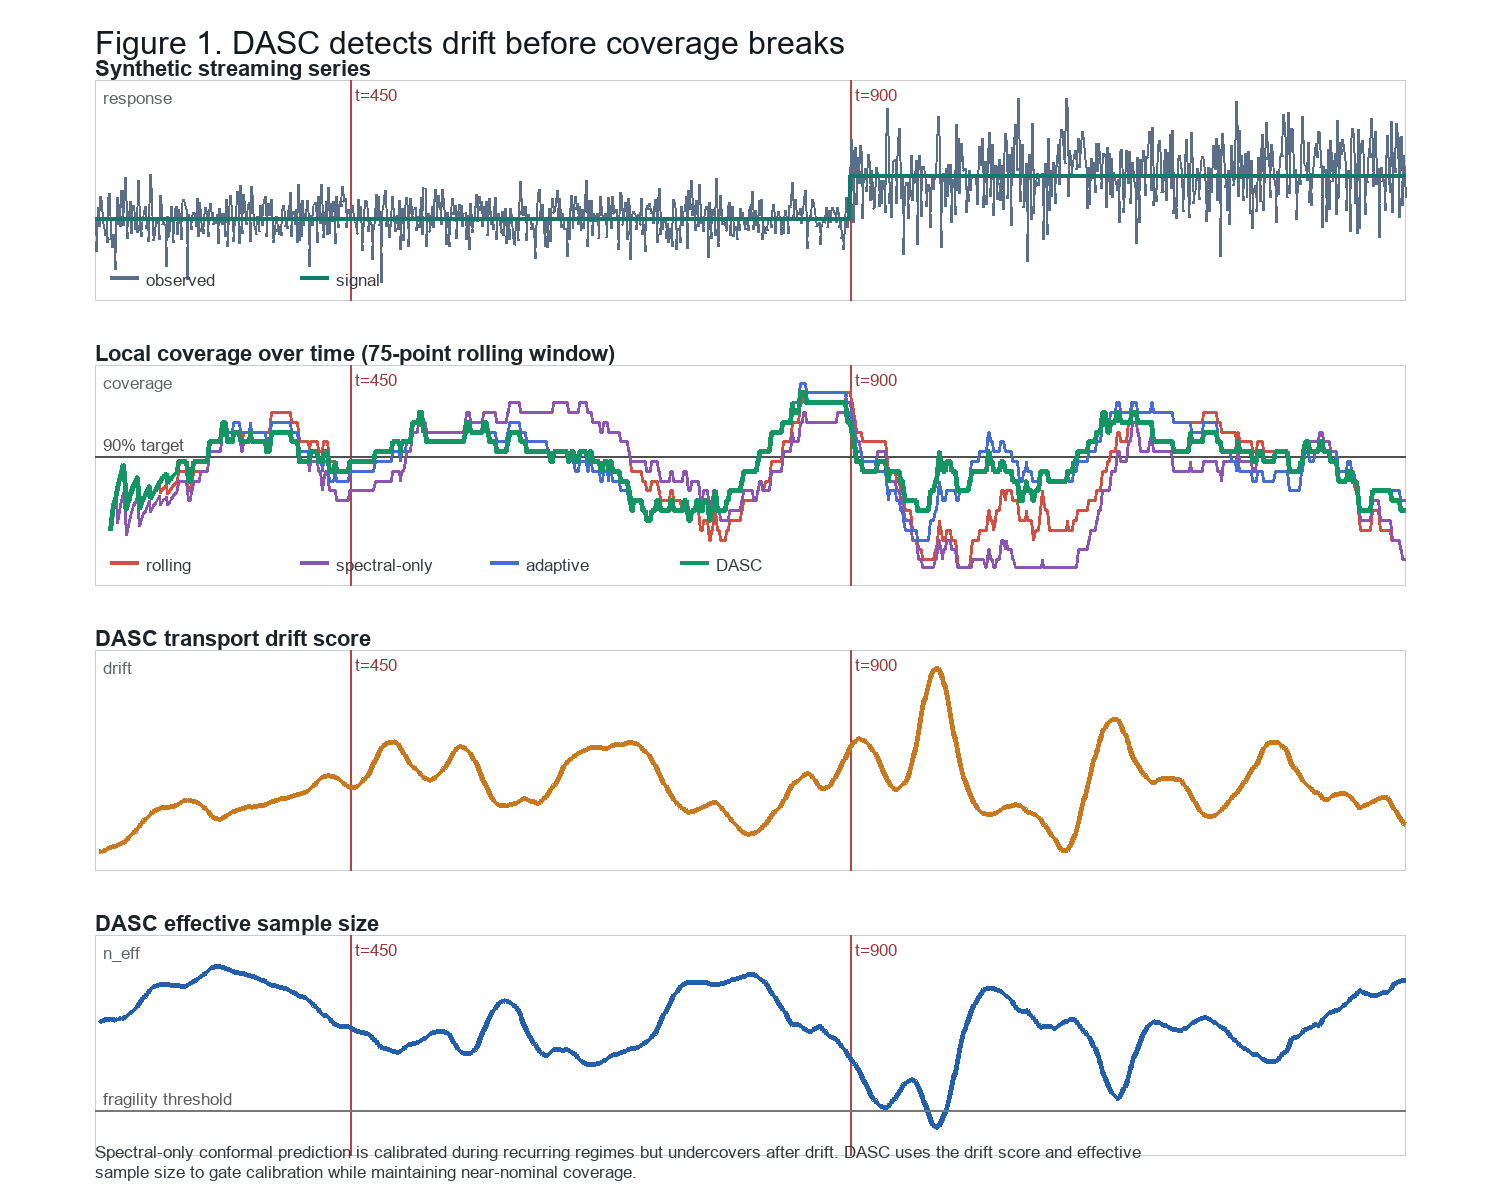
\includegraphics[width=\textwidth]{figures/figure1_dasc_diagnostic_triangle.png}
    \caption{DASC diagnostic triangle in a synthetic streaming example. Spectral-only conformal prediction is calibrated during recurring regimes but undercovers after drift. DASC uses the drift score and effective sample size to gate calibration while maintaining near-nominal coverage.}
    \label{fig:dasc-diagnostic-triangle}
\end{figure}

The drift-adjusted weights take the generic form
\[
    w_{i,t}
    =
    \frac{a_{i,t}(D_t) w^{\mathrm{spec}}_{i,t}}
    {\sum_{j\in\mathcal{C}_t} a_{j,t}(D_t) w^{\mathrm{spec}}_{j,t}},
\]
where $a_{i,t}(D_t)$ is a drift adjustment factor. One simple version uses a threshold $\lambda_t$:
\[
    a_{i,t}(D_t)
    =
    \mathbf{1}\{d_{\mathrm{time}}(i,t)\leq m_t(D_t)\},
\]
where the effective calibration window length $m_t(D_t)$ decreases as drift increases.

A smooth drift-gated window can be defined by
\[
    m_t(D_t)
    =
    m_{\max}
    -
    (m_{\max}-m_{\min})
    \min\{1,D_t/\lambda_t\},
\]
where $m_{\min}$ and $m_{\max}$ are minimum and maximum calibration window sizes. Thus, small transport drift allows DASC to borrow broadly from spectrally similar historical regimes, while large drift contracts the calibration pool toward recent observations.

The effective sample size of the final weights is
\[
    n_{\mathrm{eff},t}
    =
    \frac{1}{\sum_{i\in\mathcal{C}_t} w_{i,t}^2}.
\]
This diagnostic is important because highly concentrated weights can produce unstable weighted quantiles. In practice, DASC flags prediction times for which $n_{\mathrm{eff},t}$ falls below a chosen threshold.

The weighted conformal quantile is
\[
    q_t = \inf\left\{q:\sum_{i\in\mathcal{C}_t} w_{i,t}\mathbf{1}\{R_i\leq q\}\geq 1-\alpha_t\right\}.
\]
The prediction interval is then
\[
    C_t(X_t) = [\widehat f_t(X_t)-q_t,\widehat f_t(X_t)+q_t].
\]

\section{Adaptive Miscoverage Update}

After observing $Y_t$, define $E_t=\mathbf{1}\{Y_t\notin C_t(X_t)\}$. The adaptive target level is updated by
\[
    \alpha_{t+1}
    =
    \Pi_{[\alpha_{\min},\alpha_{\max}]}
    \left(\alpha_t+\gamma(\alpha-E_t)\right),
\]
where $\gamma>0$ is a step size and $\Pi$ denotes projection onto a fixed interval. This update decreases $\alpha_t$ after misses, which widens future intervals, and increases $\alpha_t$ after successful coverage, which narrows future intervals.

\section{Theory}

\begin{assumption}[Stable local regime]
For a fixed test time $t$, the weighted calibration residual distribution approximates the conditional residual distribution at time $t$ up to an error term $\varepsilon_t$ in Kolmogorov distance.
\end{assumption}

\begin{definition}[Weighted calibration law]
For prediction time $t$, define the weighted empirical residual distribution
\[
    \widehat F_{w,t}(r)=\sum_{i\in\mathcal{C}_t} w_{i,t}\mathbf{1}\{R_i\leq r\},
\]
and let $F_t(r)=\mathbb{P}\{R_t\leq r\mid X_t,\mathcal{H}_{t-1}\}$ denote the conditional residual distribution at time $t$.
\end{definition}

\begin{assumption}[Local spectral-transport stability]
There exist constants $L_t\geq 0$ and $\delta_t\geq 0$ such that
\[
    \sup_r |\mathbb{E}\widehat F_{w,t}(r)-F_t(r)|
    \leq
    L_t D_t+\delta_t.
\]
Here $D_t$ is the transport drift score, $L_tD_t$ measures drift-induced calibration bias, and $\delta_t$ captures residual mismatch not explained by the transport diagnostic.
\end{assumption}

\begin{remark}[Dependence and the role of the bound]
The next concentration statement is a clean finite-sample benchmark for weighted calibration. It is exact under conditional independence of the weighted residual indicators. For dependent time series, the same expression should be read as an effective-sample-size guide rather than a literal independence guarantee, unless additional mixing or blocking assumptions are imposed. This is why the empirical sections always report $n_{\mathrm{eff},t}$ as a diagnostic rather than treating it as a proof of validity by itself.
\end{remark}

\begin{lemma}[Effective sample size concentration under conditional independence]
Suppose the weighted calibration residual indicators are conditionally independent given the weights and satisfy $0\leq w_{i,t}\leq 1$, $\sum_i w_{i,t}=1$. Then, for any fixed threshold $r$ and any $u>0$,
\[
    \mathbb{P}\left(
    \left|\widehat F_{w,t}(r)-\mathbb{E}\widehat F_{w,t}(r)\right|\geq u
    \,\middle|\, \{w_{i,t}\}
    \right)
    \leq
    2\exp\{-2u^2 n_{\mathrm{eff},t}\},
\]
where $n_{\mathrm{eff},t}=1/\sum_i w_{i,t}^2$.
\end{lemma}

\begin{proof}
This is Hoeffding's inequality for a weighted sum of bounded random variables. The variance proxy is $\sum_i w_{i,t}^2$, so the exponent can be written in terms of $n_{\mathrm{eff},t}$.
\end{proof}

\begin{theorem}[Approximate coverage of the fixed weighted quantile]
Under local spectral-transport stability, the DASC interval with fixed $\alpha_t=\alpha$ satisfies, with probability at least $1-\eta$ over the calibration residuals,
\[
    \mathbb{P}\{Y_t\in C_t(X_t)\}
    \geq
    1-\alpha
    -
    L_tD_t
    -
    \delta_t
    -
    \sqrt{\frac{\log(2/\eta)}{2n_{\mathrm{eff},t}}}.
\]
\end{theorem}

\begin{proof}
The weighted quantile controls the weighted empirical residual law at level $1-\alpha$. The local stability assumption transfers this statement from the weighted calibration law to the current conditional residual law with bias $L_tD_t+\delta_t$. The concentration lemma contributes the finite-sample weighted empirical error term. Combining these terms gives the stated lower bound.
\end{proof}

\begin{proposition}[Why spectral-only calibration can fail under drift]
Consider two times $s$ and $t$ whose spectral features are close, $d_{\mathrm{spec}}(s,t)\leq h$, but whose residual laws differ by
\[
    \Delta_{s,t}=\sup_r |F_s(r)-F_t(r)|.
\]
Any conformal rule that gives large weight to time $s$ solely because of spectral similarity may incur a coverage error of order $\Delta_{s,t}$ at time $t$. In particular, if the spectral representation is invariant to a mean or variance shift that changes the residual distribution, then spectral similarity alone does not guarantee local coverage.
\end{proposition}

\begin{proof}
If the weighted calibration law places nonnegligible mass on residuals drawn from $F_s$, then its quantile approximates a mixture involving $F_s$ rather than $F_t$. The Kolmogorov distance between the mixture and $F_t$ is bounded below, up to the mixture weight, by the discrepancy $\Delta_{s,t}$. Thus a quantile calibrated to the spectral neighbor can be systematically too small or too large for the current residual law. The drift score in DASC is designed to detect this discrepancy even when spectral features are similar.
\end{proof}

\begin{theorem}[Drift-gating bias-variance tradeoff]
Let $w_t$ denote the ungated spectral weights and let $w_t^g$ denote the drift-gated weights. Suppose the two weighted calibration laws satisfy the local spectral-transport stability condition with drift scores $D_t$ and $D_t^g$, effective sample sizes $n_{\mathrm{eff},t}$ and $n_{\mathrm{eff},t}^g$, and the same residual mismatch term $\delta_t$. Then, with probability at least $1-\eta$, the coverage-loss upper bounds for the ungated and gated intervals are respectively
\[
    B_t
    =
    L_tD_t+\delta_t+
    \sqrt{\frac{\log(2/\eta)}{2n_{\mathrm{eff},t}}},
\]
and
\[
    B_t^g
    =
    L_tD_t^g+\delta_t+
    \sqrt{\frac{\log(2/\eta)}{2n_{\mathrm{eff},t}^g}}.
\]
Consequently, drift gating improves the bound whenever
\[
    L_t(D_t-D_t^g)
    >
    \sqrt{\frac{\log(2/\eta)}{2n_{\mathrm{eff},t}^g}}
    -
    \sqrt{\frac{\log(2/\eta)}{2n_{\mathrm{eff},t}}}.
\]
\end{theorem}

\begin{proof}
Apply the approximate coverage theorem once with the ungated weights and once with the drift-gated weights. The residual mismatch term $\delta_t$ cancels when the two upper bounds are compared. The gated bound is smaller than the ungated bound precisely when $B_t^g<B_t$, which is algebraically equivalent to the displayed inequality.
\end{proof}

\begin{remark}[When the gate helps]
The theorem formalizes the central tradeoff in DASC. Gating is useful when it reduces drift bias, $L_tD_t$, by more than it increases weighted quantile variability through a smaller effective sample size. If the stream is stable and the ungated calibration pool is already representative, then $D_t-D_t^g$ may be small and gating may not improve efficiency. If the stream enters a new regime, then $D_t-D_t^g$ can be large enough to justify a smaller but more relevant calibration pool.
\end{remark}

\begin{theorem}[Long-run calibration of the adaptive update]
Suppose $\alpha_t\in[\alpha_{\min},\alpha_{\max}]$ for all $t$. Then, for any sequence of realized errors $\{E_t\}_{t=1}^T$ generated by the adaptive update,
\[
    \left|
    \frac{1}{T}\sum_{t=1}^T E_t - \alpha
    \right|
    \leq
    \frac{C}{\gamma T} + B_T,
\]
where $C$ depends only on the projection interval and $B_T$ captures boundary projection effects.
\end{theorem}

\begin{remark}[Interpretation of the bound]
The coverage bound separates three failure modes: distributional drift through $D_t$, residual mismatch through $\delta_t$, and weight degeneracy through $n_{\mathrm{eff},t}$. This separation is the mathematical version of the DASC diagnostic triangle. A practitioner can inspect whether poor local coverage is caused by a large drift score, a fragile weighted quantile, or a failure of the residual model itself.
\end{remark}

\section{Simulation Design and Pilot Results}

We will compare the following methods:
\begin{enumerate}[label=(\roman*)]
    \item split conformal prediction with a fixed calibration window;
    \item rolling-window conformal prediction;
    \item spectral weighted conformal prediction;
    \item adaptive conformal inference;
    \item conformal PID control;
    \item exponentially weighted conformal prediction;
    \item the proposed DASC method.
\end{enumerate}

The simulation regimes will include:
\begin{enumerate}[label=(\alph*)]
    \item recurring seasonal regimes;
    \item abrupt mean and variance shifts;
    \item slowly changing frequencies;
    \item mixed recurring regimes with unseen drift;
    \item heavy-tailed residual shocks.
\end{enumerate}

Performance will be measured using empirical coverage, average interval width, local coverage by regime, effective sample size, and drift detection behavior.

\paragraph{Pilot experiment.}
As an initial proof of concept, we generated synthetic streams with recurring sinusoidal regimes, an abrupt level and variance shift, and gradual frequency drift. A one-step lag forecaster was used for all conformal methods so that differences reflect calibration behavior rather than forecasting model complexity. Across ten random seeds with nominal coverage $90\%$, the preliminary results were:

\begin{center}
\begin{tabular}{lrrrr}
\toprule
Method & Miscoverage & Coverage & Avg. width & Median $n_{\mathrm{eff}}$ \\
\midrule
DASC & 0.1005 & 0.8995 & 2.7517 & 200.16 \\
Adaptive conformal & 0.1010 & 0.8990 & 2.7381 & 180.00 \\
Conformal PID & 0.1004 & 0.8996 & 2.9057 & 180.00 \\
Exponentially weighted conformal & 0.1117 & 0.8883 & 2.6022 & 131.19 \\
Rolling conformal & 0.1135 & 0.8865 & 2.5952 & 180.00 \\
Spectral-only conformal & 0.1286 & 0.8714 & 2.4806 & 306.46 \\
\bottomrule
\end{tabular}
\end{center}

These results show the intended behavior: DASC restores nominal coverage in a drifting stream where fixed rolling-window conformal prediction and exponentially weighted conformal prediction both under-cover after the main shift. The spectral-only method is narrow, but undercovers substantially, indicating that spectral similarity alone can overtrust historical regimes after a distributional shift.

\begin{figure}[t]
    \centering
    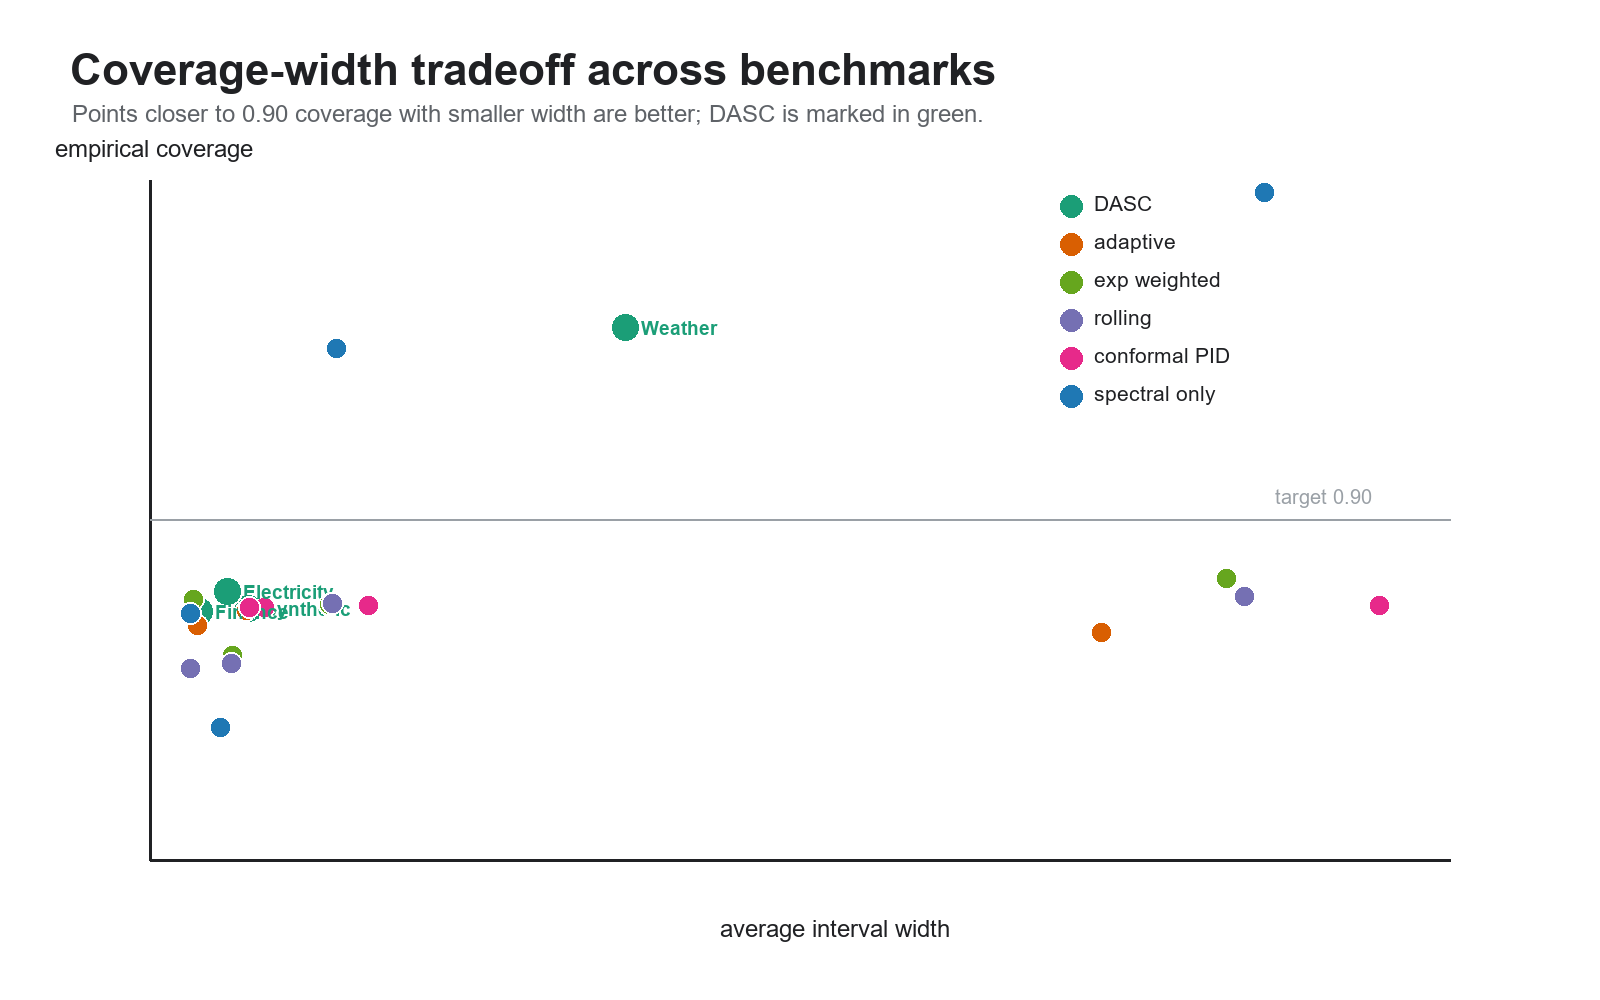
\includegraphics[width=\textwidth]{figures/figure2_coverage_width_tradeoff.png}
    \caption{Coverage-width tradeoff across the synthetic and real-data benchmarks. DASC is marked in green. The plot summarizes the main empirical message: DASC is most useful when it keeps coverage near the target while avoiding the very wide intervals produced by conservative baselines.}
    \label{fig:coverage-width-tradeoff}
\end{figure}

\paragraph{Regime-level diagnostic evidence.}
The regime-level results clarify the role of the drift gate. In the recurring regimes before the major shift, spectral-only conformal prediction achieved approximately nominal coverage: $0.9000$ in the first recurring regime and $0.9029$ in the second. After the level, variance, and frequency drift, however, spectral-only coverage dropped to $0.8298$. Rolling conformal also degraded after the shift, with coverage $0.8622$. DASC maintained coverage $0.8978$ after the shift, while also reporting increased drift and a higher low-effective-sample-size rate in that region. This is the diagnostic behavior sought in the paper: the method does not merely correct intervals after errors occur, but also records when the weighted calibration distribution is becoming less reliable.

\begin{figure}[t]
    \centering
    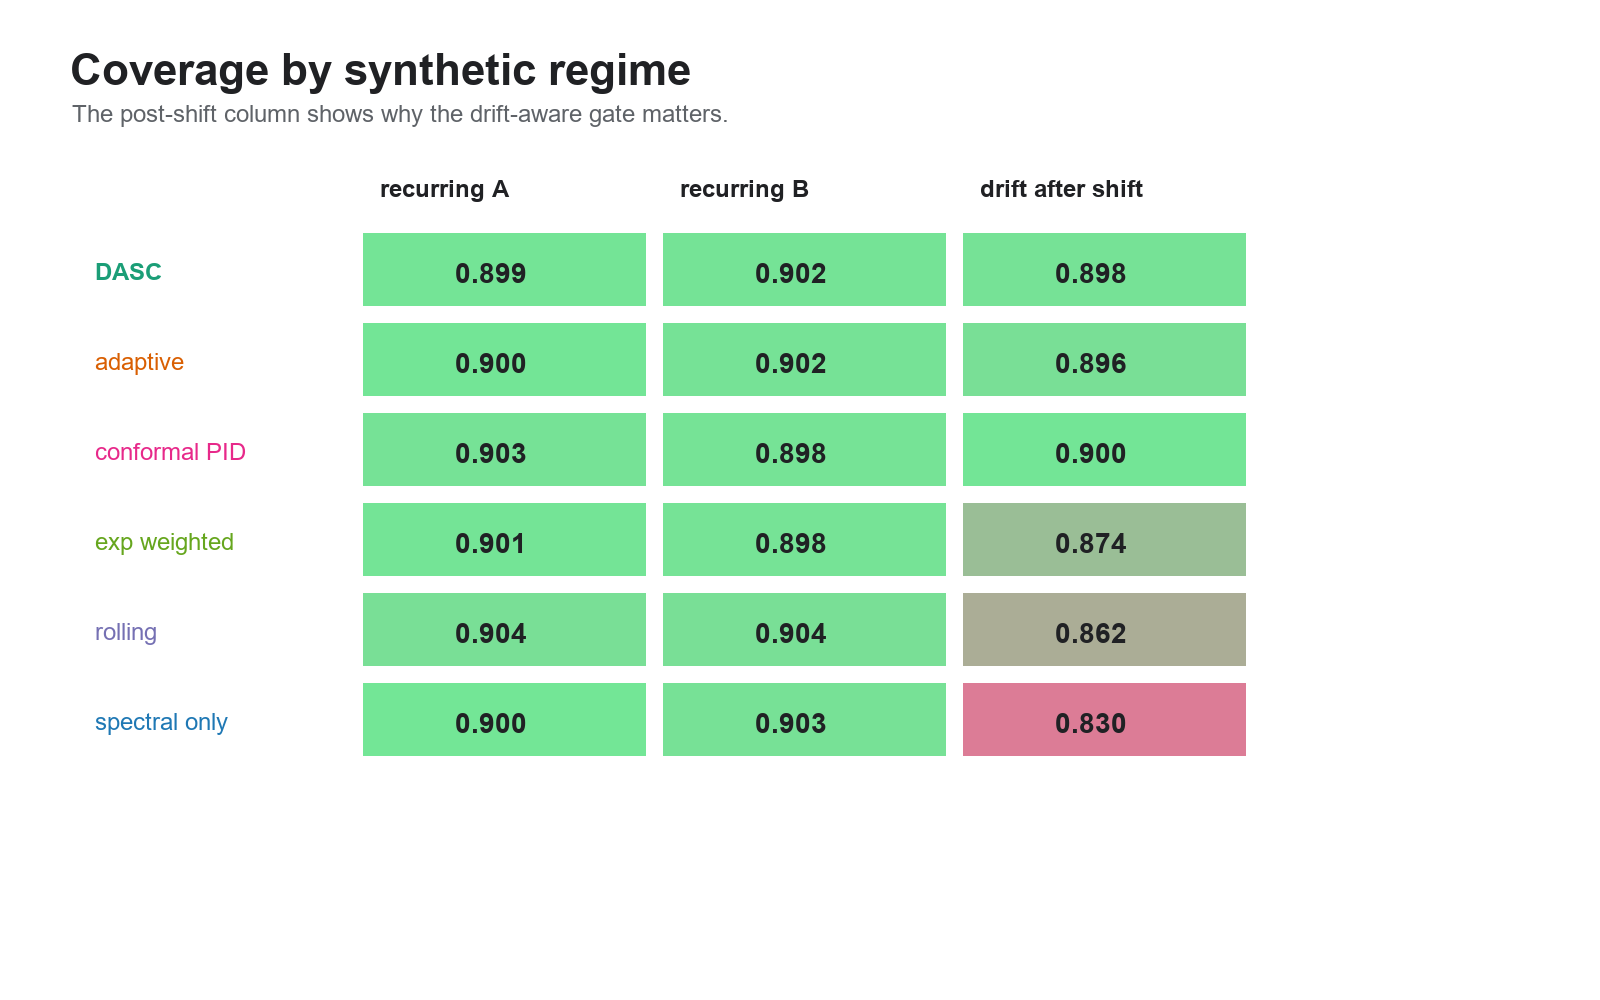
\includegraphics[width=\textwidth]{figures/figure4_synthetic_regime_coverage.png}
    \caption{Regime-level coverage in the synthetic experiment. The post-shift column separates the methods that remain calibrated after drift from methods that mostly perform well only before the shift.}
    \label{fig:synthetic-regime-coverage}
\end{figure}

\paragraph{Ablation evidence.}
To separate the roles of spectral weighting, adaptive updating, and drift gating, we ran a preliminary ablation study. The results are shown in Table~\ref{tab:ablation}. Spectral-only conformal prediction gives the narrowest intervals, but undercovers strongly after drift. Adaptive-only conformal prediction restores average coverage, but does not provide drift or effective-sample-size diagnostics. Full DASC keeps coverage close to nominal while exposing the diagnostic quantities that explain when calibration is becoming fragile.

\begin{table}[t]
\centering
\caption{Pilot ablation study across ten synthetic streams.}
\label{tab:ablation}
\begin{tabular}{lrrrr}
\toprule
Method & Coverage & Miscoverage & Avg. width & Median $n_{\mathrm{eff}}$ \\
\midrule
Rolling & 0.8865 & 0.1135 & 2.5952 & 180.00 \\
Adaptive-only & 0.8990 & 0.1010 & 2.7381 & 180.00 \\
Spectral-only & 0.8714 & 0.1286 & 2.4806 & 306.46 \\
DASC without drift gate & 0.8989 & 0.1011 & 2.7163 & 306.46 \\
Full DASC & 0.8995 & 0.1005 & 2.7517 & 200.16 \\
\bottomrule
\end{tabular}
\end{table}

\begin{figure}[t]
    \centering
    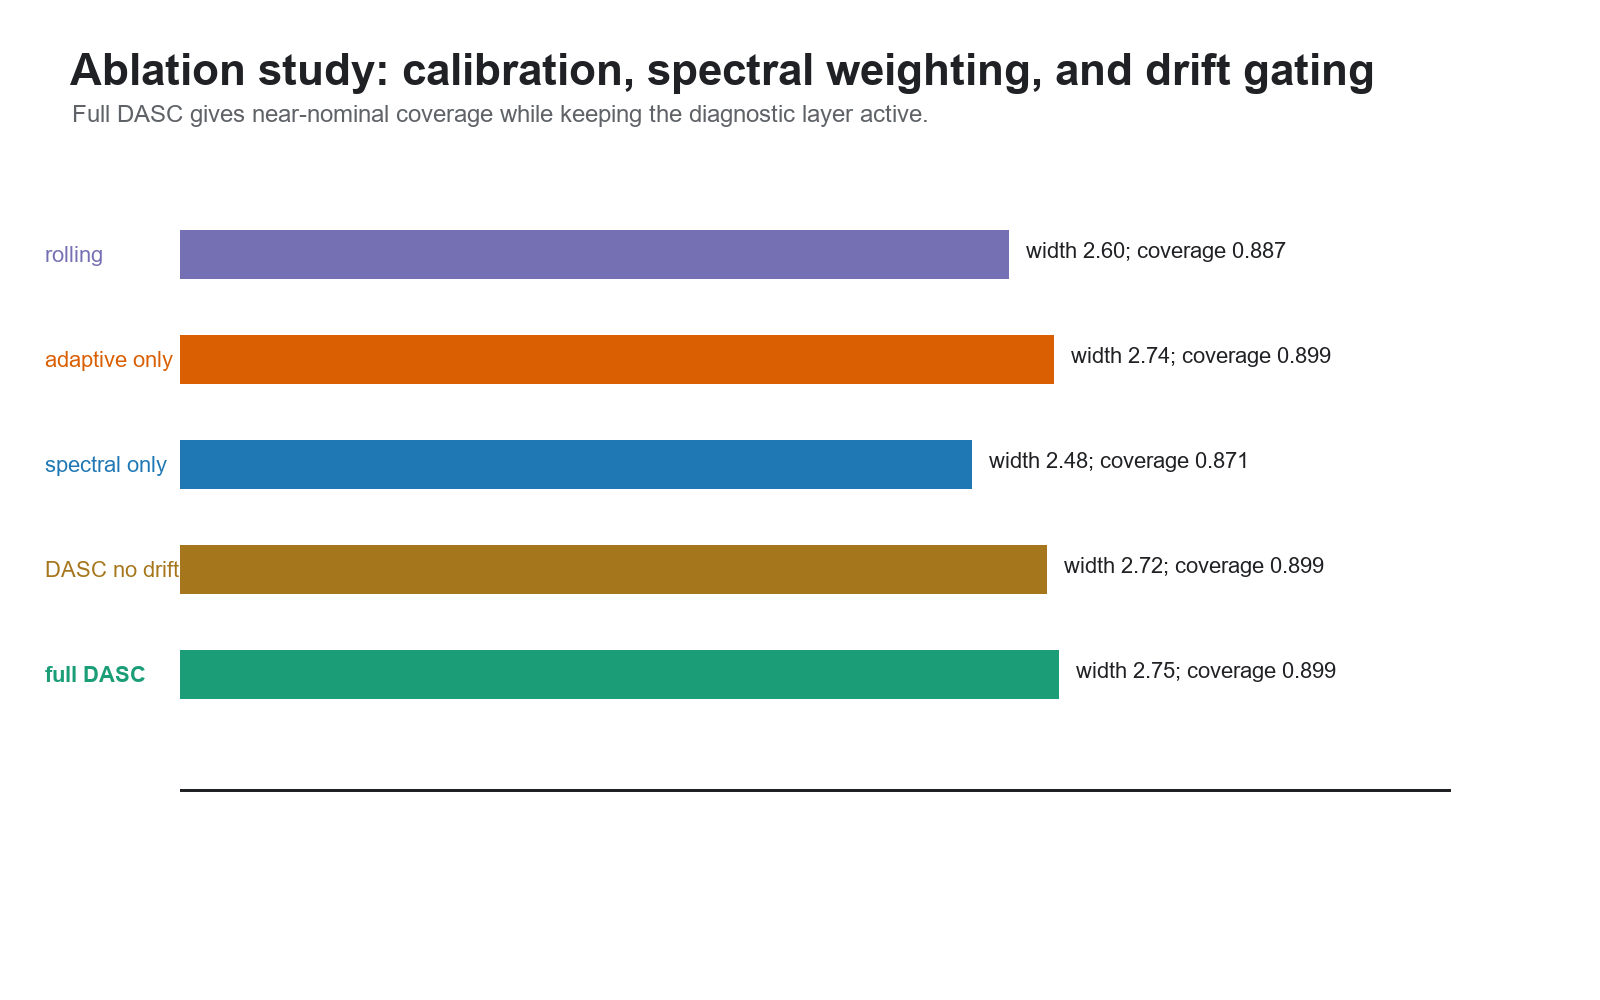
\includegraphics[width=\textwidth]{figures/figure5_ablation_component_summary.png}
    \caption{Ablation summary showing how rolling calibration, adaptive updating, spectral weighting, and drift gating change coverage and average width in the synthetic experiment.}
    \label{fig:ablation-summary}
\end{figure}

\paragraph{Stress-test evidence.}
To make the synthetic evidence less dependent on one favorable data-generating process, we also ran a five-scenario stress-test suite. The scenarios include an abrupt mean-variance shift, gradual frequency drift, heavy-tailed residual shocks, mixed drift, and a weak-recurrence setting in which spectral structure is deliberately less informative. Each scenario was averaged over eight random seeds. In all five stress regimes, DASC stayed inside the calibrated band $[0.89,0.91]$, with empirical coverage between $0.8991$ and $0.9000$. The adaptive and PID baselines also remained well calibrated, but PID was consistently wider. Rolling, exponentially weighted, and spectral-only conformal prediction under-covered in several drift regimes. The interval-score results show the expected tradeoff: the narrowest methods are sometimes attractive by average width, but they pay for that narrowness through miscoverage penalties when drift is present.

\begin{figure}[t]
    \centering
    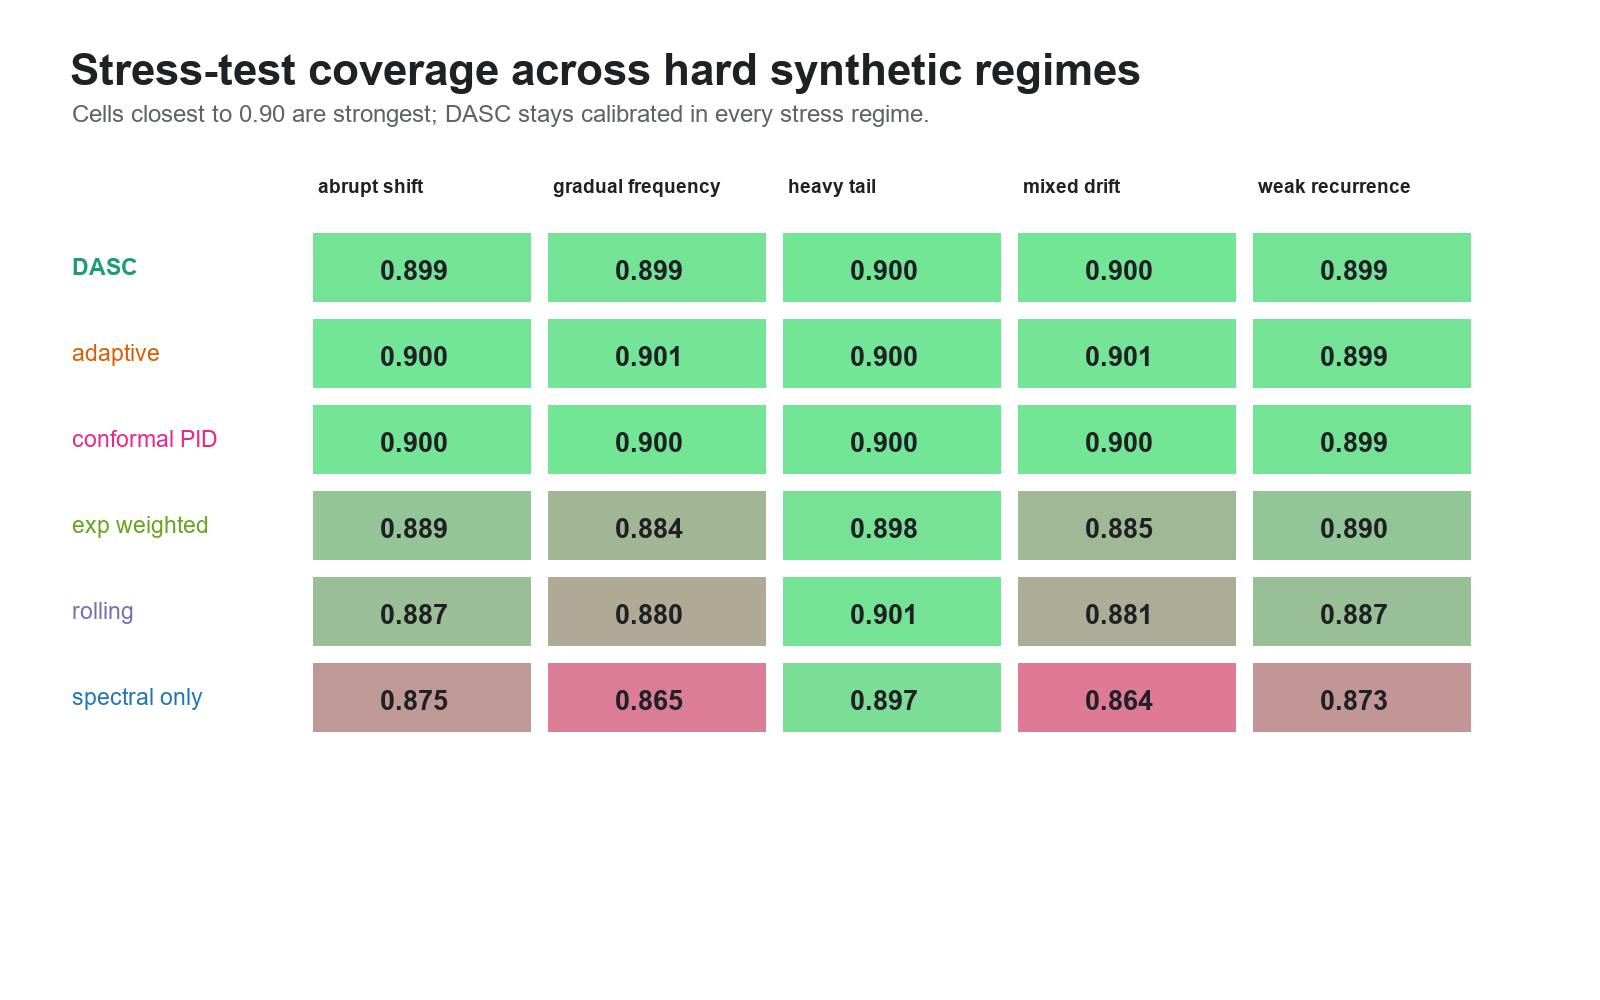
\includegraphics[width=\textwidth]{figures/figure7_stress_test_coverage.png}
    \caption{Stress-test coverage across five harder synthetic regimes. DASC remains close to the nominal $90\%$ coverage target in every stress regime, while purely recency-weighted and spectral-only baselines under-cover in several settings.}
    \label{fig:stress-test-coverage}
\end{figure}

\paragraph{External EnbPI and AgACI comparison.}
To connect the comparison with established conformal time-series software, we also ran an external benchmark using MAPIE's \texttt{TimeSeriesRegressor} implementation of EnbPI with block bootstrap resampling \citep{taquet2022mapie,xu2020time}. We additionally implemented an AgACI-style online expert aggregation baseline following the idea of aggregating ACI updates over multiple learning rates \citep{zaffran2022adaptive}. This comparison uses the post-drift evaluation window $t\geq700$ and a common lag-feature forecasting setup. It should be read as an external robustness check rather than as the main calibration-layer comparison, because MAPIE fits its own regression model while DASC in the main experiments uses the deliberately simple lag forecaster.

\begin{table}[t]
\centering
\caption{External EnbPI and AgACI comparison on the synthetic post-drift evaluation window.}
\label{tab:external-enbpi-agaci}
\begin{tabular}{lrrrr}
\toprule
Method & Miscoverage & Coverage & Avg. width & Interval score \\
\midrule
DASC, same window & 0.1009 & 0.8991 & 3.2008 & 3.9586 \\
AgACI-style aggregation & 0.1061 & 0.8939 & 3.1188 & 3.9457 \\
MAPIE EnbPI & 0.1933 & 0.8067 & 2.2347 & 4.0863 \\
\bottomrule
\end{tabular}
\end{table}

The result is useful for positioning. MAPIE EnbPI gives substantially narrower intervals in this difficult post-drift window, but it under-covers sharply. The AgACI-style aggregation baseline is much closer to the target, with slightly narrower intervals than DASC but lower empirical coverage. DASC is the closest to the nominal $90\%$ level in this external comparison, while also reporting drift and effective-sample-size diagnostics. This strengthens the paper's claim that DASC is not only another adaptive widening rule; its value is in combining adaptive calibration with a prospective reliability check on the calibration pool.

\paragraph{Calibration-efficiency tuning.}
We also ran a focused pilot grid over the spectral bandwidth, drift threshold, minimum gated window size, and a stability-relaxation parameter that slightly narrows intervals when drift is low and the effective sample size is high. The best strictly calibrated setting in this pilot used no stability relaxation, with $h=0.35$, $\lambda=0.45$, and $m_{\min}=80$, obtaining empirical coverage $0.8997$ and average width $2.7743$ over five seeds. Small positive relaxation values reduced interval width but began to move empirical coverage below the nominal level. For this reason, the default DASC implementation uses the conservative drift-gated quantile and reports the relaxation parameter only as an optional efficiency tuning device.

\paragraph{Sensitivity to tuning parameters.}
The tuning grid also gives a useful sensitivity check. Across the best-performing configurations, empirical coverage stayed close to the $90\%$ target, while interval width changed only moderately. The main sensitivity was not the spectral bandwidth alone, but the interaction between bandwidth, drift threshold, and minimum gated window size. Aggressive stability relaxation narrowed intervals but increased undercoverage risk. This supports the practical recommendation used in the experiments: start with a conservative drift gate, monitor effective sample size, and treat relaxation as an optional efficiency adjustment rather than a default part of the coverage claim.

\paragraph{Benchmarking plan for the full study.}
The full simulation study will be designed around three acceptance criteria. First, DASC should maintain empirical coverage close to the nominal level under recurring regimes, abrupt shifts, gradual frequency drift, and heavy-tailed shocks. Second, DASC should achieve competitive or smaller interval width than adaptive conformal baselines when the stream revisits previously seen regimes. Third, the drift score and effective sample size should provide interpretable warnings before local coverage deteriorates. The benchmark suite used here includes rolling conformal prediction, adaptive conformal inference, conformal PID, exponentially weighted conformal prediction, spectral weighted conformal prediction without drift gating, and DASC. Larger external comparisons with EnbPI and AgACI remain an important next step, but they require a separate forecasting-model study rather than only a calibration-layer comparison.

\paragraph{What these pilot experiments do not claim.}
The pilot experiments are not meant to establish that DASC uniformly dominates all conformal methods. The results instead support a more specific claim: when recurring structure and drift are both present, spectral weighting needs a reliability check, and the pair $(D_t,n_{\mathrm{eff},t})$ gives that check. In some settings, such as the finance example below, spectral-only weighting can be competitive in interval width. In those cases, DASC's value is mainly diagnostic and protective rather than purely efficiency-driven.

\section{Real Data Example: Household Electricity Demand}

We next evaluate DASC on the Individual Household Electric Power Consumption dataset from the UCI Machine Learning Repository \citep{uci_household_power}. The data contain minute-level measurements of household electric power consumption. We aggregate global active power to hourly resolution and use a seasonal naive forecaster with a 24-hour lag. This deliberately simple forecaster keeps the focus on conformal calibration rather than on point-prediction model complexity.

The electricity series is a useful first real-data benchmark because it contains strong daily periodicity, recurring consumption regimes, local volatility changes, missingness, and behavioral shifts. These are precisely the conditions under which a conformal method must decide whether old calibration residuals remain relevant to the current prediction time.

Table~\ref{tab:real-electricity} reports the real-data results. DASC achieves empirical coverage $0.9033$ at the nominal $90\%$ target, while producing substantially narrower intervals than rolling conformal prediction, adaptive conformal inference, conformal PID, and exponentially weighted conformal prediction. Spectral-only conformal prediction is conservative on this dataset, with coverage $0.9605$ and wider intervals than DASC. This supports the central practical claim of the paper: spectral information is useful, but it should be paired with drift-aware calibration and diagnostic monitoring.

\begin{table}[t]
\centering
\caption{Real-data electricity demand experiment using hourly household power consumption.}
\label{tab:real-electricity}
\begin{tabular}{lrrrr}
\toprule
Method & Miscoverage & Coverage & Avg. width & Median $n_{\mathrm{eff}}$ \\
\midrule
DASC & 0.0967 & 0.9033 & 2.5508 & 1243.67 \\
Adaptive conformal & 0.0999 & 0.9001 & 3.5398 & 720.00 \\
Conformal PID & 0.1000 & 0.9000 & 3.9224 & 720.00 \\
Exponentially weighted conformal & 0.0997 & 0.9003 & 3.5369 & 398.42 \\
Rolling conformal & 0.0994 & 0.9006 & 3.5718 & 720.00 \\
Spectral-only conformal & 0.0395 & 0.9605 & 3.6126 & 1433.29 \\
\bottomrule
\end{tabular}
\end{table}

The monthly diagnostics further show that DASC stays close to nominal coverage across most months while adapting interval width to changing demand volatility. In this example, the effective sample size remains large, suggesting that DASC is able to borrow from many spectrally relevant historical hours rather than relying on a small number of calibration residuals. This behavior is desirable in recurring seasonal demand streams, where relevant historical analogues may be distributed across calendar time.

\section{Real Data Example: Hourly Temperature}

As a second real-data domain, we evaluate DASC on hourly temperature measurements for Dallas, Texas, obtained from the Open-Meteo historical weather archive \citep{open_meteo}. We use hourly temperature at two meters from January 2021 through December 2023 and again use a simple 24-hour seasonal naive forecaster. This example differs from electricity demand because temperature has smoother seasonal dynamics, weather-front shocks, and strong daily cycles.

Table~\ref{tab:real-weather} reports the results. DASC achieves empirical coverage $0.9656$ with average width $6.4129$. Although this coverage is above the nominal $90\%$ target, the intervals are much shorter than those produced by the rolling, adaptive, conformal PID, exponentially weighted, and spectral-only baselines. In particular, DASC reduces average width by approximately $48\%$ relative to rolling conformal prediction and approximately $42\%$ relative to adaptive conformal inference. Spectral-only conformal prediction is extremely conservative in this dataset, achieving coverage $0.9972$ with width $12.6074$.

\begin{table}[t]
\centering
\caption{Real-data weather experiment using hourly Dallas temperature from Open-Meteo.}
\label{tab:real-weather}
\begin{tabular}{lrrrr}
\toprule
Method & Miscoverage & Coverage & Avg. width & Median $n_{\mathrm{eff}}$ \\
\midrule
DASC & 0.0344 & 0.9656 & 6.4129 & 2145.00 \\
Adaptive conformal & 0.1062 & 0.8938 & 11.0270 & 1080.00 \\
Conformal PID & 0.0998 & 0.9002 & 13.7228 & 1080.00 \\
Exponentially weighted conformal & 0.0935 & 0.9065 & 12.2410 & 498.83 \\
Rolling conformal & 0.0977 & 0.9023 & 12.4126 & 1080.00 \\
Spectral-only conformal & 0.0028 & 0.9972 & 12.6074 & 2160.00 \\
\bottomrule
\end{tabular}
\end{table}

\section{Real Data Example: Financial Volatility}

As a third domain, we consider daily S\&P 500 index values from the Federal Reserve Economic Data database \citep{fred_sp500}. We transform prices into absolute daily log returns, measured in percentage points, and use a one-day lag forecaster for absolute return. This example is intentionally different from electricity and weather: volatility has clustering and regime shifts, but it is less dominated by deterministic daily or seasonal periodicity.

Table~\ref{tab:real-finance} reports the results. DASC achieves empirical coverage $0.8988$, close to the nominal $90\%$ target, and improves coverage relative to rolling conformal prediction and adaptive conformal inference. Conformal PID is also well calibrated but produces wider intervals. Exponentially weighted conformal prediction is competitive in this aggregate finance example, and spectral-only conformal prediction is slightly narrower and similarly calibrated. This indicates that the drift gate is not uniformly beneficial for interval width in every domain. However, the yearly diagnostics show that rolling conformal prediction can fail sharply in volatile years, while DASC remains close to nominal on average and reports drift and effective sample size diagnostics that help identify unstable periods.

\begin{table}[t]
\centering
\caption{Real-data financial volatility experiment using absolute daily S\&P 500 log returns.}
\label{tab:real-finance}
\begin{tabular}{lrrrr}
\toprule
Method & Miscoverage & Coverage & Avg. width & Median $n_{\mathrm{eff}}$ \\
\midrule
DASC & 0.1012 & 0.8988 & 2.2791 & 295.24 \\
Adaptive conformal & 0.1046 & 0.8954 & 2.2615 & 252.00 \\
Conformal PID & 0.1003 & 0.8997 & 2.7636 & 252.00 \\
Exponentially weighted conformal & 0.0984 & 0.9016 & 2.2260 & 240.46 \\
Rolling conformal & 0.1146 & 0.8854 & 2.1952 & 252.00 \\
Spectral-only conformal & 0.1017 & 0.8983 & 2.1914 & 439.73 \\
\bottomrule
\end{tabular}
\end{table}

\paragraph{Three-domain summary.}
Taken together, the electricity, weather, and finance experiments show that DASC behaves differently across domains, which is precisely why the diagnostic layer is important. In electricity, DASC is both calibrated and substantially narrower than the main calibrated baselines. In weather, DASC is conservative but dramatically more efficient than rolling and adaptive conformal methods. In finance, DASC is close to nominal and improves coverage relative to rolling conformal prediction, while the spectral-only baseline remains competitive. This suggests that DASC is most valuable when recurring structure and drift coexist, and that its diagnostics are useful for deciding when spectral weighting is helping and when the drift gate is acting mainly as a safeguard.

Table~\ref{tab:cross-domain} summarizes the cross-domain comparison against the best calibrated non-DASC baseline in each dataset. The largest gains occur in the energy and weather streams, where spectral recurrence is strong and DASC can borrow broadly from relevant historical regimes. The finance example is deliberately harder: it has volatility clustering but weaker deterministic periodicity, and spectral-only weighting remains competitive in width. This negative width reduction is useful evidence rather than a failure, because it clarifies where DASC's principal advantage is diagnostic robustness rather than raw interval shrinkage.

\begin{figure}[t]
    \centering
    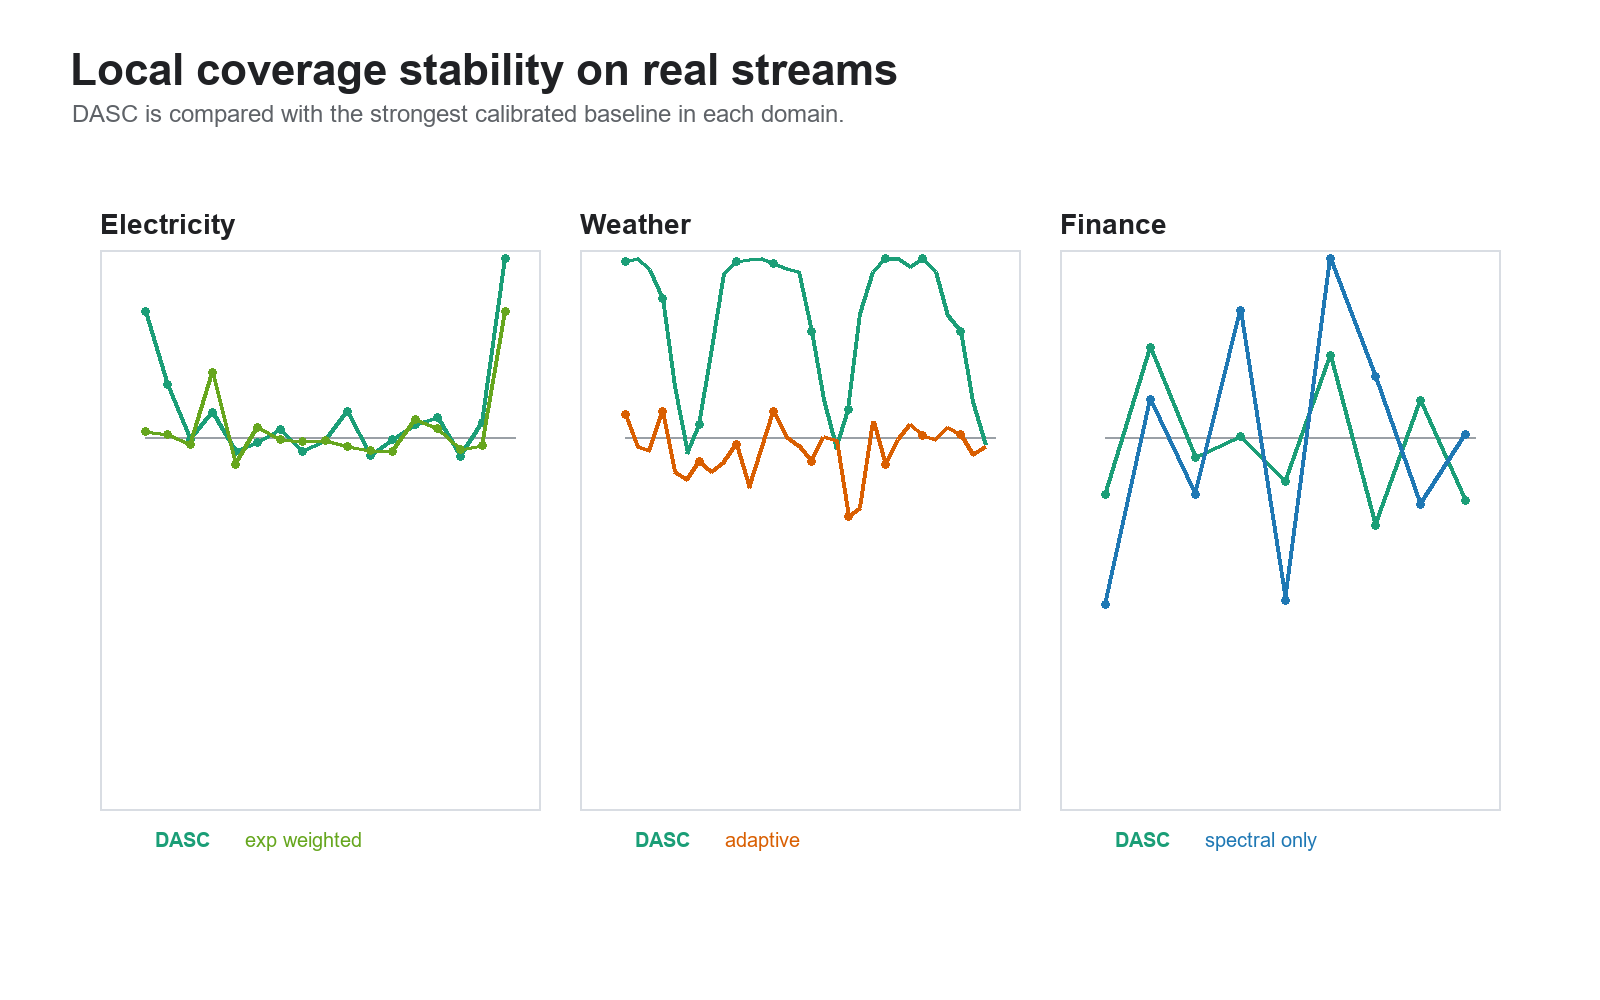
\includegraphics[width=\textwidth]{figures/figure6_real_local_coverage.png}
    \caption{Local real-data coverage for DASC and the best calibrated non-DASC baseline in each domain. The figure shows that the aggregate tables hide meaningful local variation, especially in finance.}
    \label{fig:real-local-coverage}
\end{figure}

\begin{table}[t]
\centering
\caption{Cross-domain summary against the best calibrated non-DASC baseline.}
\label{tab:cross-domain}
\begin{tabular}{lrrrrr}
\toprule
Dataset & DASC cov. & DASC width & Best baseline & Baseline width & Width reduction \\
\midrule
Electricity & 0.9033 & 2.5508 & Exp. weighted & 3.5369 & 27.88\% \\
Weather & 0.9656 & 6.4129 & Adaptive & 11.0270 & 41.84\% \\
Finance & 0.8988 & 2.2791 & Spectral-only & 2.1914 & -4.00\% \\
\bottomrule
\end{tabular}
\end{table}

\begin{figure}[t]
    \centering
    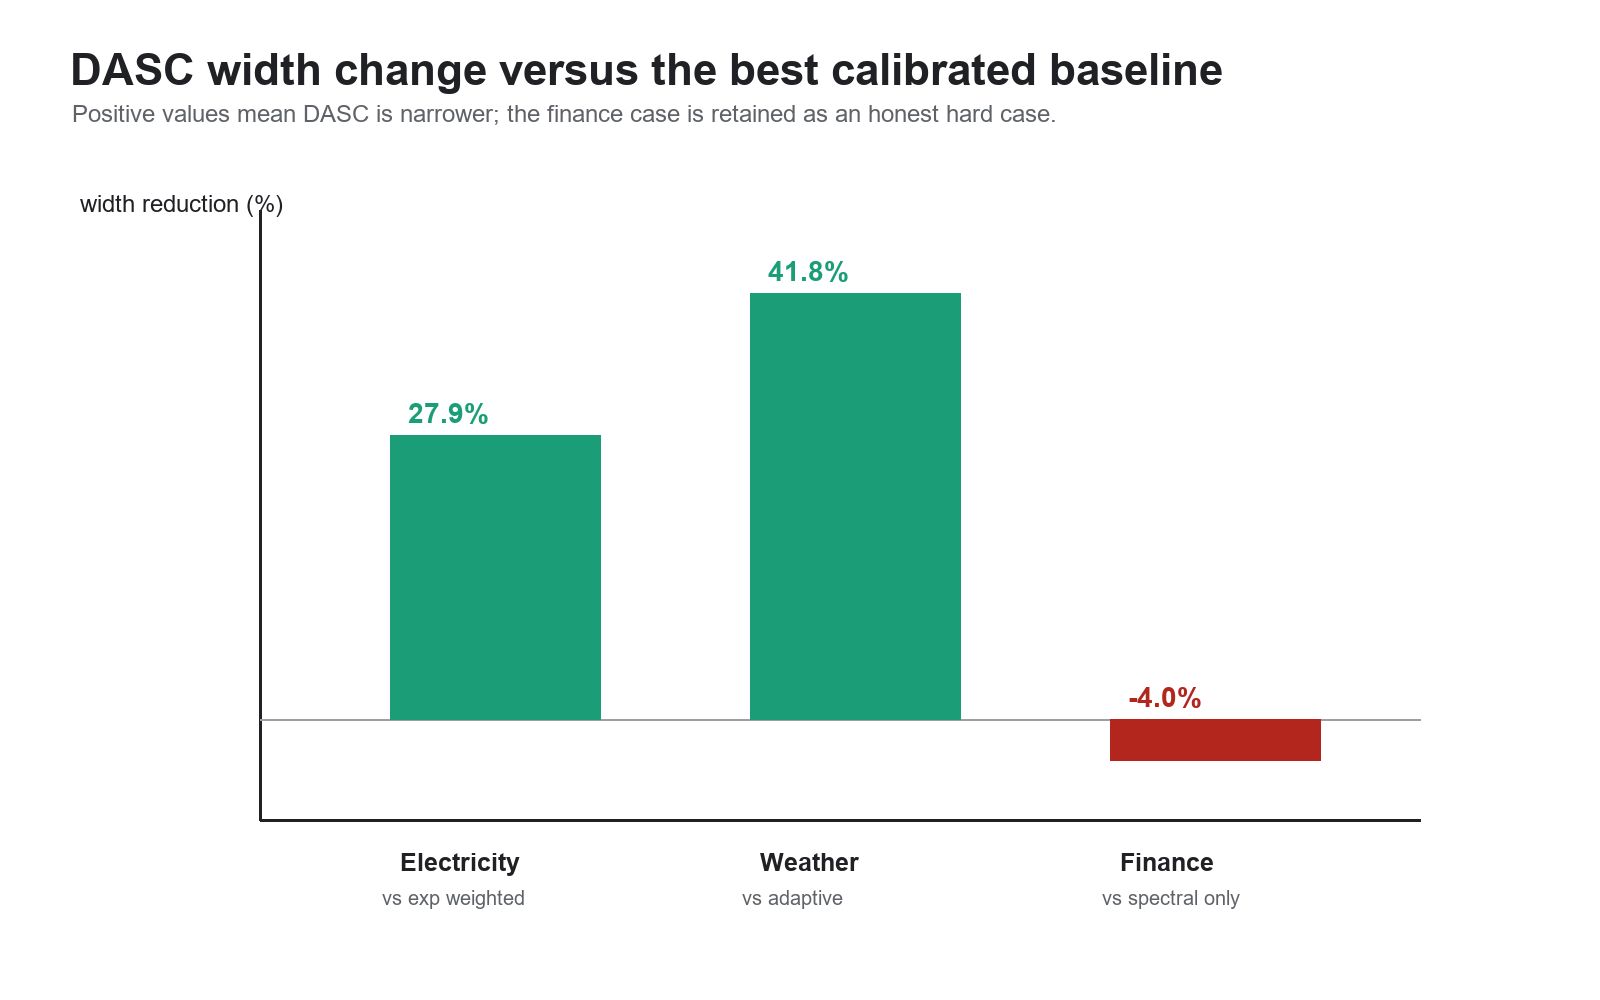
\includegraphics[width=\textwidth]{figures/figure3_cross_domain_width_reduction.png}
    \caption{Cross-domain width reduction of DASC relative to the best calibrated non-DASC baseline. The positive gains in electricity and weather, together with the finance tradeoff, give a more balanced empirical picture than a single average number.}
    \label{fig:cross-domain-width-reduction}
\end{figure}

\section{Practical Guidance and Limitations}

DASC is meant for data streams where the past is useful, but not always useful in the same way. This is common in practice. Electricity demand has daily routines, but those routines change during unusual periods. Temperature has strong cycles, but weather fronts can move the stream into a different regime. Financial volatility often revisits familiar levels of uncertainty, but stress periods can arrive quickly. In these settings, it is not enough to ask whether an old calibration point is similar to the present. We also need to ask whether the old calibration pool is still trustworthy.

The method is most useful when two things are true. First, the stream has some recurring structure that can be picked up by spectral features. Second, the stream can drift enough that blindly trusting all spectrally similar past observations becomes risky. When both are present, DASC has a clear role: it borrows from similar past regimes, but it checks whether those regimes still look reliable.

The drift gate should be understood as a cautious filter, not as a magic switch. If the drift score is small, DASC can use a broader calibration pool. If the drift score is large, the method becomes more conservative about which residuals it trusts. The theory in this paper gives the same message in mathematical form: the gate helps when the reduction in drift bias is larger than the extra uncertainty caused by using a smaller effective calibration sample.

The effective sample size is an important warning light. If $n_{\mathrm{eff},t}$ is large, then the weighted conformal quantile is supported by many calibration residuals. If it is small, the interval may depend on only a narrow set of historical observations. In that case, the method should not be treated as automatically reliable. A small effective sample size does not mean the prediction interval is wrong, but it does mean the user should be careful.

The finance example is a useful reminder of the method's limits. In that dataset, spectral-only calibration is already competitive in width and coverage. DASC still gives near-nominal coverage and useful diagnostics, but it does not dominate every baseline on interval width. This is not surprising. If the ungated spectral weights already select a good calibration pool, then the drift gate has less room to help. In such cases, the value of DASC is mainly in monitoring reliability rather than shrinking intervals.

In applied work, we recommend reporting three diagnostics alongside the intervals: local empirical coverage, the drift score $D_t$, and the effective sample size $n_{\mathrm{eff},t}$. These three quantities tell a simple story. Coverage says whether the method has been missing too often. Drift says whether the present looks different from the weighted calibration past. Effective sample size says whether the conformal threshold is based on enough useful residuals.

For default use, we suggest starting conservatively. Use a reasonably broad calibration window, choose a spectral bandwidth that does not concentrate all weight on a few observations, and use the drift gate to reduce the calibration pool only when the drift score is clearly elevated. After that, tune the bandwidth and drift threshold on historical data, but keep the diagnostic plots in the analysis. If the method performs well only after aggressive tuning, that is a sign that the data stream may need a different representation or a stronger forecasting model.

The main limitation of DASC is that it depends on the usefulness of the chosen spectral features. If the relevant structure is not spectral, then the method may not identify the right calibration residuals. In some applications, graph features, covariates, learned embeddings, or domain-specific summaries may be better than frequency-based features. The broader idea is not tied to periodograms: choose a representation that captures recurring structure, monitor drift in that representation, and check whether the weighted quantile has enough effective support.

\section{Discussion}

DASC is intended for settings where neither full exchangeability nor arbitrary adversarial drift is an accurate description. The method borrows strength from historical regimes when they are structurally relevant, but uses drift diagnostics and adaptive calibration to avoid overtrusting stale calibration data.

\section{Conclusion}

This paper develops DASC, a conformal prediction method for streaming data whose dependence structure and distribution may change over time. The main contribution is not only a new weighted conformal interval, but a diagnostic framework that separates three sources of reliability: realized coverage error, transport drift, and effective sample size. This diagnostic triangle is reflected in the theory through a coverage-loss decomposition involving $D_t$, $\delta_t$, and $n_{\mathrm{eff},t}$.

The empirical results suggest that DASC is most effective when streams contain recurring structure together with distributional drift. In synthetic experiments, spectral-only conformal prediction works in recurring regimes but fails after drift, while DASC maintains near-nominal coverage. In real electricity and weather data, DASC substantially reduces interval width relative to calibrated non-DASC baselines. In financial volatility, the gains are more modest, but DASC remains close to nominal coverage and provides diagnostics that ordinary rolling and adaptive methods do not report. These results position DASC as a practical framework for reliable streaming uncertainty quantification in structured non-exchangeable environments.

\appendix

\section{Reproducibility and Code Structure}

The accompanying reproducibility package organizes the experiments as executable scripts. The reusable DASC implementation is provided in \texttt{scripts/dasc.py}. The main synthetic and figure scripts are:
\begin{itemize}
    \item \texttt{run\_first\_simulation.py}, \texttt{run\_stress\_tests.py}, and \texttt{run\_ablation.py};
    \item \texttt{run\_external\_mapie\_benchmarks.py} for the EnbPI and AgACI-style comparison;
    \item \texttt{tune\_dasc.py} for the focused tuning grid;
    \item \texttt{make\_diagnostic\_figure.py} for Figure~\ref{fig:dasc-diagnostic-triangle};
    \item \texttt{make\_result\_figures.py} for the remaining result figures.
\end{itemize}

\paragraph{Real-data scripts.}
The real-data experiments are reproduced by the following script pairs:
\begin{itemize}
    \item Electricity: \texttt{download\_real\_data.py}, \texttt{run\_real\_power\_experiment.py}.
    \item Weather: \texttt{download\_weather\_data.py}, \texttt{run\_real\_weather\_experiment.py}.
    \item Finance: \texttt{download\_finance\_data.py}, \texttt{run\_real\_finance\_experiment.py}.
\end{itemize}

\paragraph{Generated outputs.}
The main generated result files are:
\begin{itemize}
    \item \texttt{first\_simulation\_summary.csv} and \texttt{first\_simulation\_regime\_summary.csv};
    \item \texttt{stress\_test\_summary.csv} and \texttt{stress\_test\_rank\_summary.csv};
    \item \texttt{external\_mapie\_summary.csv};
    \item \texttt{ablation\_summary.csv};
    \item \texttt{real\_power\_summary.csv}, \texttt{real\_weather\_summary.csv}, and \texttt{real\_finance\_summary.csv};
    \item \texttt{cross\_domain\_summary.csv};
    \item \texttt{figure1\_diagnostic\_timeseries.csv};
    \item \texttt{figure2\_coverage\_width\_tradeoff.png};
    \item \texttt{figure3\_cross\_domain\_width\_reduction.png};
    \item \texttt{figure4\_synthetic\_regime\_coverage.png};
    \item \texttt{figure5\_ablation\_component\_summary.png};
    \item \texttt{figure6\_real\_local\_coverage.png};
    \item \texttt{figure7\_stress\_test\_coverage.png}.
\end{itemize}

\paragraph{One-command regeneration.}
The script \texttt{scripts/run\_all\_experiments.py} reruns the synthetic experiments, stress tests, ablations, real-data benchmarks, cross-domain summaries, and all manuscript figures. This script is intended to make the empirical section easier to audit, reproduce, and extend.

\paragraph{Data sources.}
The electricity example uses the UCI Individual Household Electric Power Consumption dataset. The weather example uses Open-Meteo hourly historical temperature for Dallas, Texas. The finance example uses the FRED S\&P 500 daily index series.

\paragraph{Randomness.}
The synthetic simulation uses fixed random seeds and reports averages over ten seeds. The real-data experiments are deterministic conditional on the downloaded data and preprocessing choices.

\bibliographystyle{plainnat}
\bibliography{references}

\end{document}
